Based on our specification, we created a design for the application's user interface. The user interface had to support the use cases specified in section \ref{sec:use_cases}, although not all features required in the use cases were included in the design. The goal of the design was to include the features listed as \textit{Must have} and \textit{Should have} in the MoSCoW analysis, but still take the other features into account. This was done to ensure that the most important aspects of the use cases would be satisfied in the design, while also having designed for some of the desirable but less important features.

In the following sections, we describe wireframes each showing a view of a page on our web application. Furthermore, each section includes a description of which use cases and features each page satisfies.

\section{Wireframe for Solving Exercises}
Figures \ref{fig:wfExerciseInstructions} and \ref{fig:wfExerciseResult} show wireframes for the page intended for solving exercises.

% primary use cases
% solve exercises
\begin{figure}[H]
	\frame{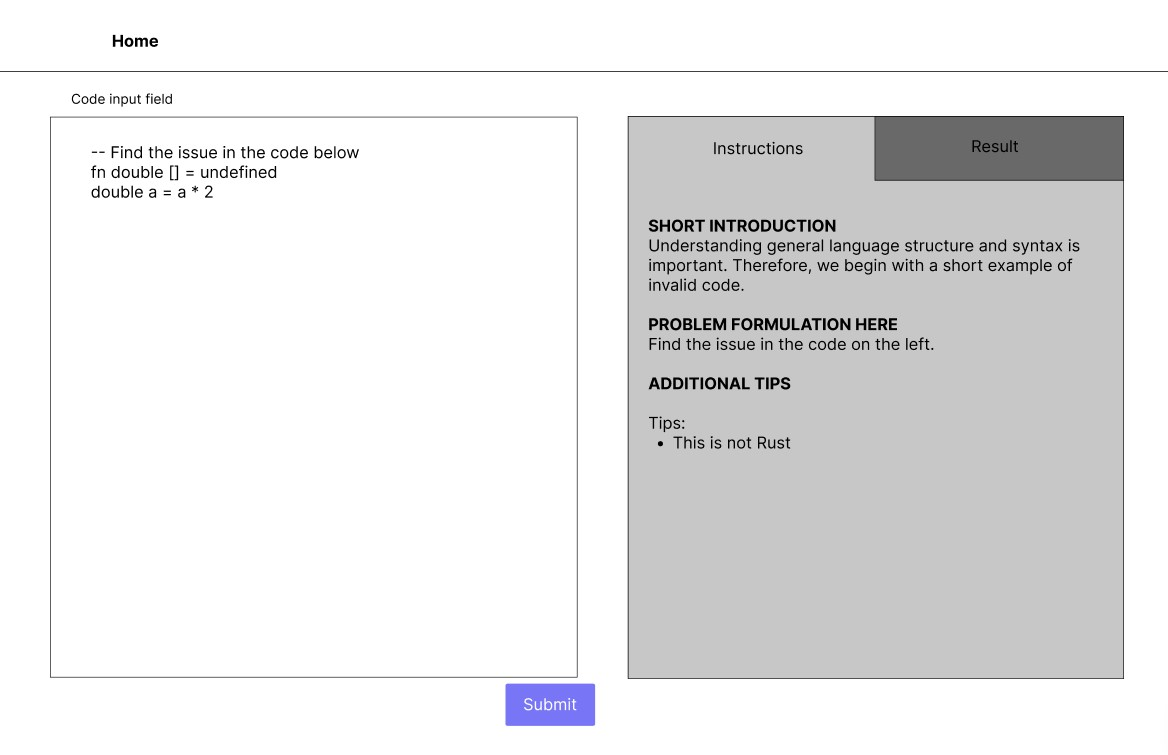
\includegraphics[scale=0.5]{WireframeSolveInstruction.jpg}}
	\centering
	\caption{Wireframe for solving an exercise showing the instructions tab}
	\label{fig:wfExerciseInstructions}
\end{figure}

\begin{figure}[H]
	\frame{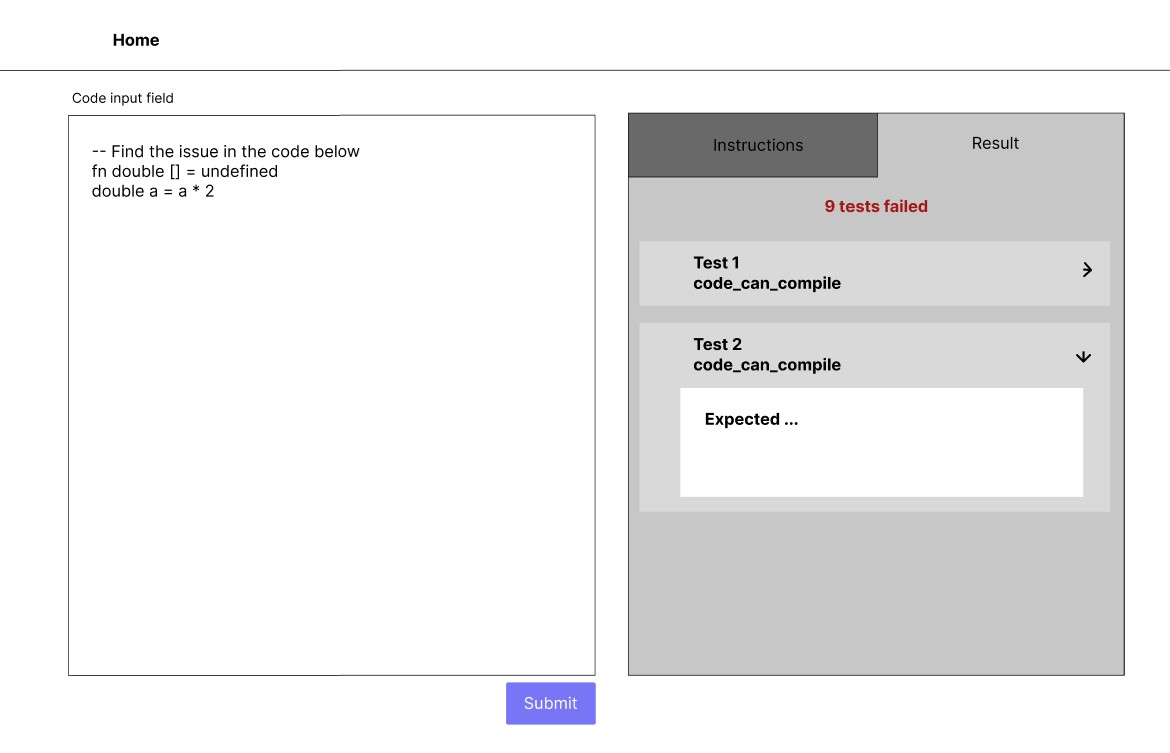
\includegraphics[scale=0.5]{WireframeSolveResult.jpg}}
	\centering
	\caption{Wireframe for solving an exercise showing the result tab}
	\label{fig:wfExerciseResult}
\end{figure}

Both figure \ref{fig:wfExerciseInstructions} and figure \ref{fig:wfExerciseResult} show a text input field to the left, which is where the user can write code to solve an exercise.
The only difference between the two figures is which tab is open.
Figure \ref{fig:wfExerciseInstructions} shows what page looks like when the instructions tab is open, while figure \ref{fig:wfExerciseResult} shows what the page looks like with the result tab open.
The instructions tab displays the exercise instructions to the user.
The result tab opens after submitting the code and shows whether it passed the tests for the exercise.
This design satisfies the requirements that an exercise should have a description, and that a user should be able to submit and verify their code an exercise submission, as stated in the use case \textbf{Solve exercises}.

\section{Wireframe for Browsing}
Since the design for the page displayed in figure \ref{fig:wfExercise} does not satisfy the entirety of the \textbf{Solve exercises} use case, we have designed a separate page to browse exercises as well as sessions and syllabi. The page structure for all of these are similar, and therefore we only show an example of a page for browsing syllabi.

% Structure of creating sessions and syllabi
\begin{figure}[H]
    \frame{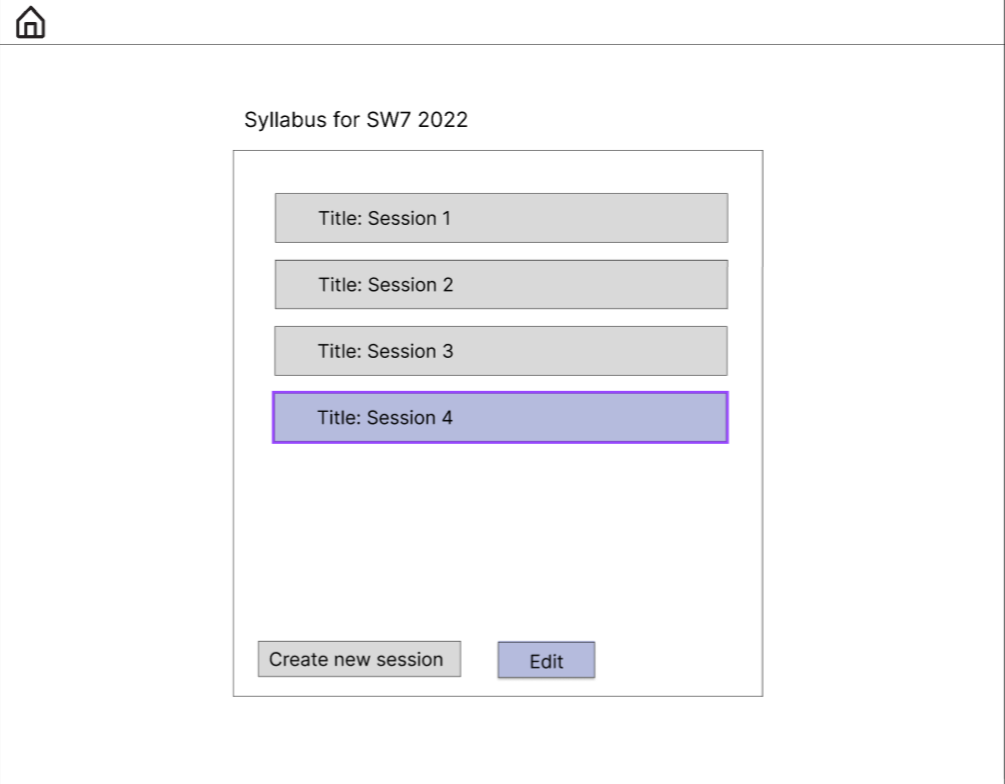
\includegraphics[scale=0.4]{browseSyllabus.png}}
    \centering
    \caption{Wireframe for browsing a syllabus}
    \label{fig:wfSyllabus}
\end{figure}
Note that the buttons related to creating new items or updating items in the list will only be available to the lecturer. The items shown in the list correspond to the page the user is on. If the user is browsing syllabi, the items contained in the list will be syllabi. If the user is browsing sessions, the list will contain sessions, and similarly for exercises. This design satisfies the use case \textbf{Solve exercises} by letting users choose sessions and exercises. Additionally, it also satisfies part of the use case \textbf{Create exercises} by providing the ability to create and edit syllabi and exercises.

\section{Wireframe for Creating an Exercise}
The wireframe in figure \ref{fig:wfProblem}, shows the page that the lecturer will see, when the create exercise button when browsing exercises.
% create exercises
\begin{figure}[H]
	\frame{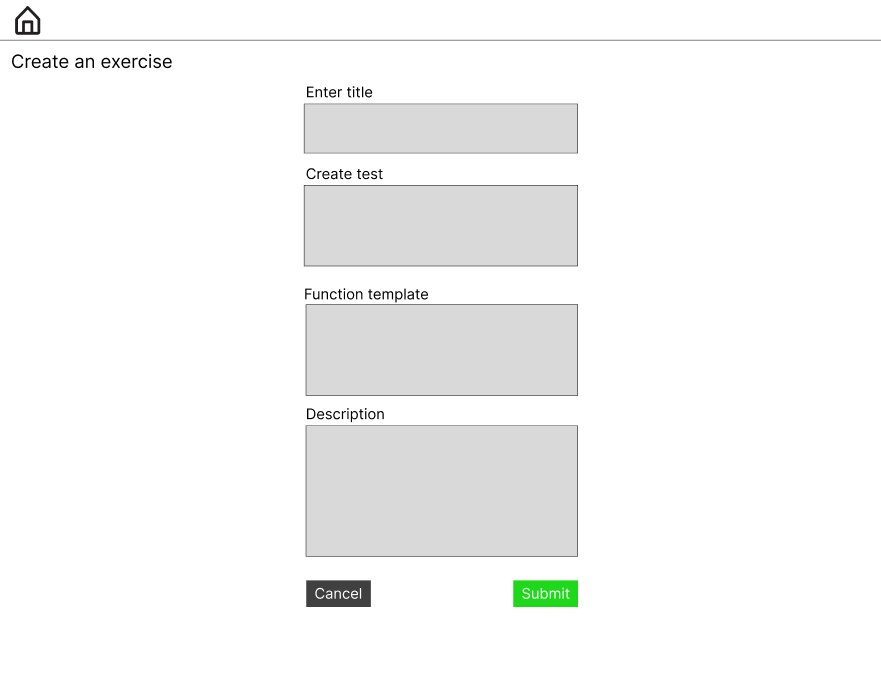
\includegraphics[scale=0.65]{createProblem.jpg}}
	\centering
	\caption{Wireframe for creating a problem}
	\label{fig:wfProblem}
\end{figure}

This page allows the lecturer to create an exercise with a title, test, function template, and description.
By typing Hspec tests in the test input field, the lecturer can specify conditions that must be satisfied for a submission to be considered a valid solution.
The function template field allows the lecturer to define a template for the exercise, which will load into the code editor upon opening the exercise.
This satisfies the remaining requirements of the use case \textbf{Create exercises}.

With the design of the user interface in place, we now move on to describing an overview of the system as a whole.
